\documentclass[a4paper]{article}
\usepackage[utf8]{inputenc}
\usepackage{vntex}
\usepackage{a4wide,amssymb,epsfig,latexsym,multicol,array,hhline,fancyhdr}
\usepackage{booktabs}
\usepackage{amsmath}
\usepackage{lastpage}
\usepackage[lined,boxed,commentsnumbered]{algorithm2e}
\usepackage{enumerate}
\usepackage{color}
\usepackage{graphicx}
\usepackage{array}
\usepackage{tabularx, caption}
\usepackage{multirow}
\usepackage[framemethod=tikz]{mdframed}
\usepackage{multicol}
\usepackage{rotating}
\usepackage{graphics}
\usepackage{geometry}
\usepackage{setspace}
\usepackage{epsfig}
\usepackage{tikz}
\usepackage{float}
\usepackage{listings}
\usepackage{url}
\usetikzlibrary{arrows,arrows.meta,shapes.geometric,shapes.misc,positioning,fit,calc}
\usepackage{hyperref}
\hypersetup{urlcolor=blue,linkcolor=blue,citecolor=black,colorlinks=true}

\def\UrlBreaks{\do\/\do-\do_}

\geometry{
    a4paper,
    left=20mm,
    right=20mm,
    top=25mm,
    bottom=25mm
}

\setlength{\headheight}{40pt}
\pagestyle{fancy}
\fancyhead{}
\fancyhead[L]{
 \begin{tabular}{rl}
    \begin{picture}(25,15)(0,0)
    \put(0,-8){
\includegraphics[width=8mm, height=8mm]{logoITSGUsmall.png}}
   \end{picture}&
	\begin{tabular}{l}
		\textbf{\bf \ttfamily Trường Đại học Sài Gòn}\\
		\textbf{\bf \ttfamily Khoa Công Nghệ Thông Tin}
	\end{tabular} 	
 \end{tabular}
}
\fancyhead[R]{
	\begin{tabular}{r}
		\scriptsize \bf \ttfamily ĐỒ ÁN CÔNG NGHỆ PHẦN MỀM \\
		\scriptsize \bf \ttfamily ASSIGNMENT 2 -- BREWLITE
	\end{tabular}  
}
\fancyfoot{}
\fancyfoot[L]{\scriptsize \ttfamily Báo cáo Cá nhân: Nguyễn Tuấn Khôi -- Phân hệ: Chi tiết sản phẩm \& Tùy chọn món}
\fancyfoot[R]{\scriptsize \ttfamily Trang {\thepage}/\pageref{LastPage}}
\renewcommand{\headrulewidth}{0.3pt}
\renewcommand{\footrulewidth}{0.3pt}

\lstset{
  language=bash,
  basicstyle=\scriptsize\ttfamily,
  keywordstyle=\color{blue}\bfseries,
  commentstyle=\color{gray}\itshape,
  stringstyle=\color{red},
  numbers=left,
  numberstyle=\tiny\color{gray},
  stepnumber=1,
  numbersep=6pt,
  backgroundcolor=\color{white},
  showspaces=false,
  showstringspaces=false,
  showtabs=false,
  frame=single,
  tabsize=2,
  captionpos=b,
  breaklines=true,
  breakatwhitespace=false
}

\begin{document}

% ==================== TRANG BÌA ====================
\begin{titlepage}
\thispagestyle{empty}
\begin{singlespace}
\begin{center}
{\large \textbf{TRƯỜNG ĐẠI HỌC SÀI GÒN}} \\
{\large \textbf{KHOA CÔNG NGHỆ THÔNG TIN}} \\
\textbf{BỘ MÔN CÔNG NGHỆ PHẦN MỀM} \\
------o0o------
\end{center}

\vspace{0.4cm}
\begin{center}

\includegraphics[width=2.8cm]{logoITSGU.png}
\end{center}
\vspace{0.4cm}

\begin{center}
\begin{tabular}{c}
	\multicolumn{1}{l}{\textbf{{\Large BÀI TẬP LỚN: CÔNG NGHỆ PHẦN MỀM}}}\\
	\vspace{0.05cm}\\
	\hline
	\\
	\multicolumn{1}{l}{\textbf{{\large ASSIGNMENT 2: REQUIREMENTS TO DEPLOYMENT}}}\\
	\vspace{0.15cm}\\
	\textbf{{\LARGE HỆ THỐNG CÀ PHÊ BREWLITE}}\\
	\vspace{0.15cm}\\
	\textbf{{\Large BÁO CÁO CÁ NHÂN: NGUYỄN TUẤN KHÔI}}\\
	\vspace{0.1cm}\\
	\textbf{{\normalsize Màn hình \& Luồng nghiệp vụ: "Chi tiết sản phẩm \& Tùy chọn món"}}\\
	\\
	\hline
\end{tabular}
\end{center}

\vspace{0.8cm}

\begin{center}
\begin{tabular}{rll}
\textbf{GVHD:} & ThS. Từ Lãng Phiêu & \\
\vspace{0.1cm}
\textbf{SV thực hiện:} & \textbf{Nguyễn Tuấn Khôi} & \\
\vspace{0.1cm}
\textbf{Phân công:} & Màn hình \& Luồng "Chi tiết sản phẩm" & \\
\vspace{0.1cm}
\textbf{Mã yêu cầu:} & FR-03, NFR-01, NFR-02 & \\
\textbf{Học kỳ:} & I -- Năm học 2026--2027 & \\
\end{tabular}
\end{center}

\vfill
\begin{center}
{\small \textbf{TP. HỒ CHÍ MINH, THÁNG 11/2026}}
\end{center}
\end{singlespace}
\end{titlepage}

\thispagestyle{empty}
\newpage

\pagenumbering{roman}
\tableofcontents
\newpage

\pagenumbering{arabic}
\onehalfspacing

% ==================== PHẦN 1 ====================
\section{Tổng quan Bối cảnh, Phân công Nhiệm vụ và Đặc tả Yêu cầu (SRS)}

\subsection{Bối cảnh Nghiệp vụ Phân hệ Chi tiết Sản phẩm trong BrewLite}
Trong lĩnh vực kinh doanh đồ uống và dịch vụ F\&B (Food \& Beverage), thức uống không phải là một mặt hàng cố định nguyên khối mà luôn đi kèm với nhu cầu cá nhân hóa cao độ của người tiêu dùng:
\begin{itemize}
    \item \textbf{Cá nhân hóa kích cỡ (Size):} Khách hàng có nhu cầu lựa chọn các dung tích ly khác nhau (Size S: 350ml, Size M: 500ml, Size L: 700ml) tương ứng với mức phụ thu giá cụ thể.
    \item \textbf{Tùy biến món kèm (Add-on Toppings):} Khách hàng có sở thích thêm các loại topping đa dạng (thạch cà phê, trân châu hoàng kim, kem phô mai mặn...) làm gia tăng giá trị trung bình trên mỗi đơn hàng (Average Order Value - AOV).
    \item \textbf{Định lượng khẩu vị cá nhân (Portions):} Khách hàng cần chọn tỷ lệ đường (100\%, 70\%, 50\%, 30\%, 0\%) và tỷ lệ đá (100\%, 70\%, 50\%, đá riêng, không đá).
    \item \textbf{Tính toán giá tiền tức thời (Real-time Dynamic Pricing):} Khi người dùng thay đổi bất kỳ lựa chọn nào hoặc điều chỉnh số lượng, hệ thống phải cập nhật tức thời tổng tiền minh bạch ngay trên nút hành động, loại trừ độ trễ và đem lại trải nghiệm mua hàng tiện lợi.
\end{itemize}

\subsection{Bảng Phân công Trách nhiệm Nhóm và Vị trí của Thành viên 2}
Bảng phân chia trách nhiệm 5 thành viên trong đồ án môn học Công nghệ Phần mềm:

\begin{table}[H]
\centering
\small
\begin{tabularx}{\textwidth}{|c|p{3.8cm}|p{3.5cm}|X|}
\hline
\textbf{STT} & \textbf{Thành viên} & \textbf{Luồng / Màn hình} & \textbf{Trách nhiệm chính} \\ \hline
1 & Trần Vĩnh Thọ Lân & Menu sản phẩm & Task 1.1 Bối cảnh \& Phạm vi, API \texttt{GET /products} \\ \hline
\textbf{2} & \textbf{Nguyễn Tuấn Khôi} & \textbf{Chi tiết sản phẩm} & \textbf{Đặc tả SRS Tùy chọn, 5 sơ đồ UML, API \texttt{GET /products/:id}, Frontend Next.js Modal} \\ \hline
3 & Thành viên 3 & Giỏ hàng \& Đặt đơn & Quản lý State giỏ hàng, API \texttt{POST /orders}, DB Transaction \\ \hline
4 & Phan Vũ Việt Quang & Thanh toán \& Xác nhận & Task 1.3 Use-case thanh toán, Idempotency, API \texttt{POST /payments} \\ \hline
5 & Thành viên 5 & Đăng ký \& Đăng nhập & NFR Bảo mật, mã hóa bcrypt, API JWT Auth, Docker \\ \hline
\end{tabularx}
\caption{Bảng phân công trách nhiệm 5 thành viên trong hệ thống BrewLite}
\label{tab:team_roles}
\end{table}

Danh mục các nhiệm vụ cụ thể do \textbf{Thành viên 2} trực tiếp đảm nhận:
\begin{enumerate}
    \item \textbf{Soạn thảo Đặc tả Yêu cầu Phần mềm (SRS):} Đặc tả chi tiết các yêu cầu chức năng (FR-03.1 đến FR-03.6), yêu cầu phi chức năng (NFR-01, NFR-02), quy tắc nghiệp vụ (BR-01 đến BR-05), từ điển dữ liệu tại \nolinkurl{docs/requirements/srs-product-options.md}.
    \item \textbf{Thiết kế hệ thống 5 Sơ đồ UML chuẩn hóa:}
    \begin{itemize}
        \item \textit{Use Case Diagram:} Sơ đồ phân hệ Chi tiết sản phẩm \& Tùy chọn món (\nolinkurl{usecase-detail.puml}).
        \item \textit{Activity Diagram:} Sơ đồ luồng xem món, chọn Size S/M/L, Topping và tính giá tự động qua 4 swimlanes (\nolinkurl{activity-detail.puml}).
        \item \textit{Sequence Diagram:} Sơ đồ tuần tự gọi API \texttt{GET /products/:id} và luồng tính giá tại Client (\nolinkurl{sequence-detail.puml}).
        \item \textit{Class Diagram:} Sơ đồ lớp lĩnh vực mô hình hóa các lớp \texttt{ProductOption}, \texttt{SizeOption}, \texttt{Topping}, \texttt{ProductCustomization} và DTOs (\nolinkurl{class-product-option.puml}).
        \item \textit{Deployment Diagram:} Sơ đồ cấu trúc lưu trữ dữ liệu sản phẩm trong CSDL PostgreSQL 16 (\nolinkurl{deployment-product-db.puml}).
    \end{itemize}
    \item \textbf{Hiện thực Mã nguồn Frontend \& Backend:}
    \begin{itemize}
        \item Xây dựng Component Frontend Next.js: \nolinkurl{apps/web/src/components/ProductDetailModal.tsx} và thuật toán tính giá \nolinkurl{apps/web/src/utils/price-calculator.ts}.
        \item Xây dựng Backend NestJS API: \nolinkurl{apps/api/src/products/} với endpoint \texttt{GET /products/:id} và \texttt{POST /products/:id/calculate-price}.
    \end{itemize}
    \item \textbf{Kiểm thử tự động (Automated Unit Test):} Viết trọn vẹn bộ test case cho Service và Controller đạt tỷ lệ pass \textbf{13/13 tests (100\%)}.
    \item \textbf{Cập nhật Ma trận truy vết (Traceability Matrix):} Đồng bộ hóa toàn diện mã yêu cầu FR-03 tại \nolinkurl{docs/traceability-matrix.md}.
\end{enumerate}

\subsection{Quy tắc Nghiệp vụ và Công thức Tính giá Tự động (Business Rules)}
Các quy tắc cốt lõi điều chỉnh hoạt động của phân hệ:
\begin{itemize}
    \item \textbf{BR-01 (Kích cỡ mặc định):} Khi mở modal, Size M luôn được kích hoạt mặc định với phụ thu bằng $0$ VNĐ. Size S có phụ thu $-5.000$đ (hoặc $0$đ tùy sản phẩm), Size L có phụ thu $+10.000$đ.
    \item \textbf{BR-02 (Ràng buộc Topping):} Khách hàng được chọn tối đa 5 loại topping cho 1 ly. Topping có tồn kho bằng 0 sẽ bị khóa vô hiệu hóa (\texttt{disabled}).
    \item \textbf{BR-03 (Công thức tính giá thời gian thực):}
    $$\text{UnitPrice} = \text{BasePrice} + \text{SizeExtraPrice} + \sum_{i=1}^{k} \text{ToppingPrice}_i$$
    $$\text{TotalPrice} = \text{UnitPrice} \times \text{Quantity}$$
    \item \textbf{BR-04 (Kiểm soát số lượng):} Số lượng đặt tối thiểu là 1 ly và không được vượt quá số lượng tồn kho khả dụng của sản phẩm.
\end{itemize}

% ==================== PHẦN 2 ====================
\section{Bộ 5 Sơ đồ UML Đảm nhận (System Modeling \& Architecture)}

\subsection{Use Case Diagram: Chi tiết Sản phẩm \& Tùy chọn Món}
Sơ đồ Use Case phân hệ mô tả các chức năng cốt lõi của màn hình chi tiết, quan hệ \texttt{<<include>>} với kiểm tra tồn kho và tính giá, và các quan hệ \texttt{<<extend>>} đối với các thao tác tùy chọn không bắt buộc.

\begin{figure}[H]
\centering
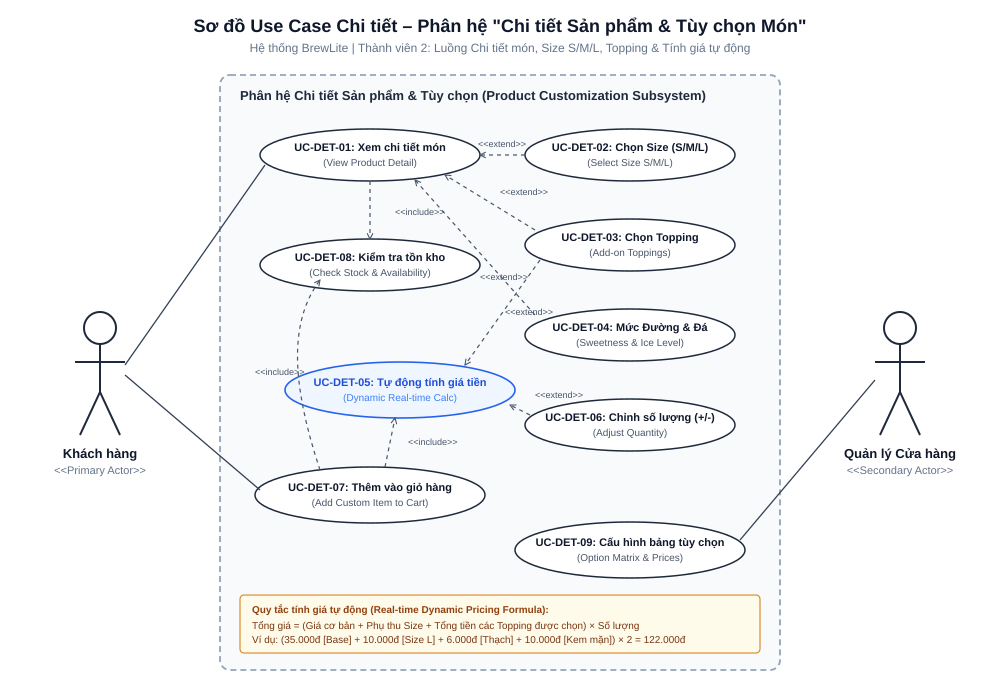
\includegraphics[width=0.92\textwidth]{../diagrams/usecase-detail.svg}
\caption{Sơ đồ Use Case Phân hệ Chi tiết Sản phẩm \& Tùy chọn Món (usecase-detail)}
\label{fig:usecase_detail}
\end{figure}

\subsection{Activity Diagram: Luồng Xem Món, Chọn Size, Topping và Tính Giá Tự Động}
Sơ đồ hoạt động được phân chia theo 4 Swimlanes rõ ràng: \textbf{Khách hàng (Customer)}, \textbf{Frontend (Next.js Modal)}, \textbf{Backend API (NestJS)} và \textbf{Database (PostgreSQL)}. Sơ đồ thể hiện chu trình lặp tương tác người dùng và hàm tính giá Client-side không độ trễ.

\begin{figure}[H]
\centering
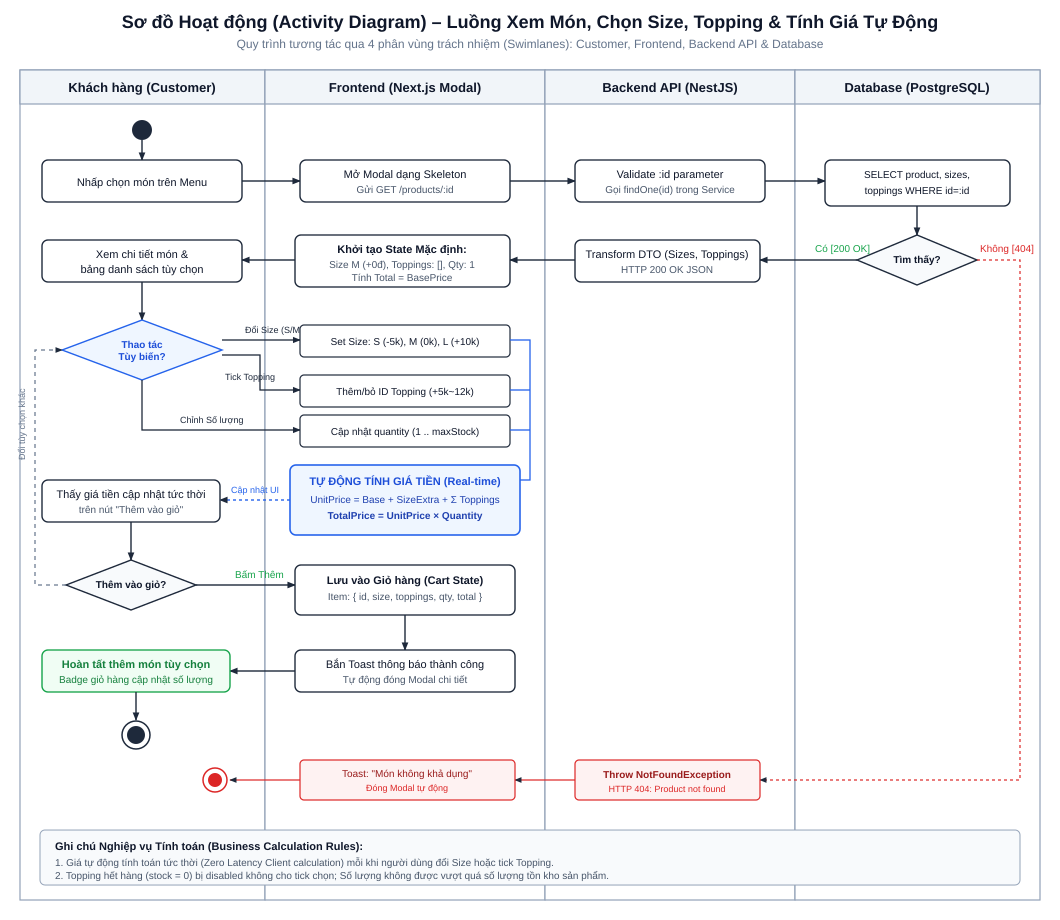
\includegraphics[width=0.95\textwidth]{../diagrams/activity-detail.svg}
\caption{Sơ đồ Hoạt động Luồng Xem Món, Chọn Size/Topping \& Tính Giá Tự Động (activity-detail)}
\label{fig:activity_detail}
\end{figure}

\subsection{Sequence Diagram: Sơ đồ Gọi API Lấy Chi Tiết Sản Phẩm (GET /products/:id)}
Sơ đồ tuần tự thể hiện tương tác giữa 5 thành phần: Customer, Next.js UI, ProductsController, ProductsService và Prisma / PostgreSQL. Sơ đồ xử lý trọn vẹn nhánh thành công (200 OK) và các nhánh lỗi (400 Bad Request, 404 Not Found, 500 Server Error).

\begin{figure}[H]
\centering
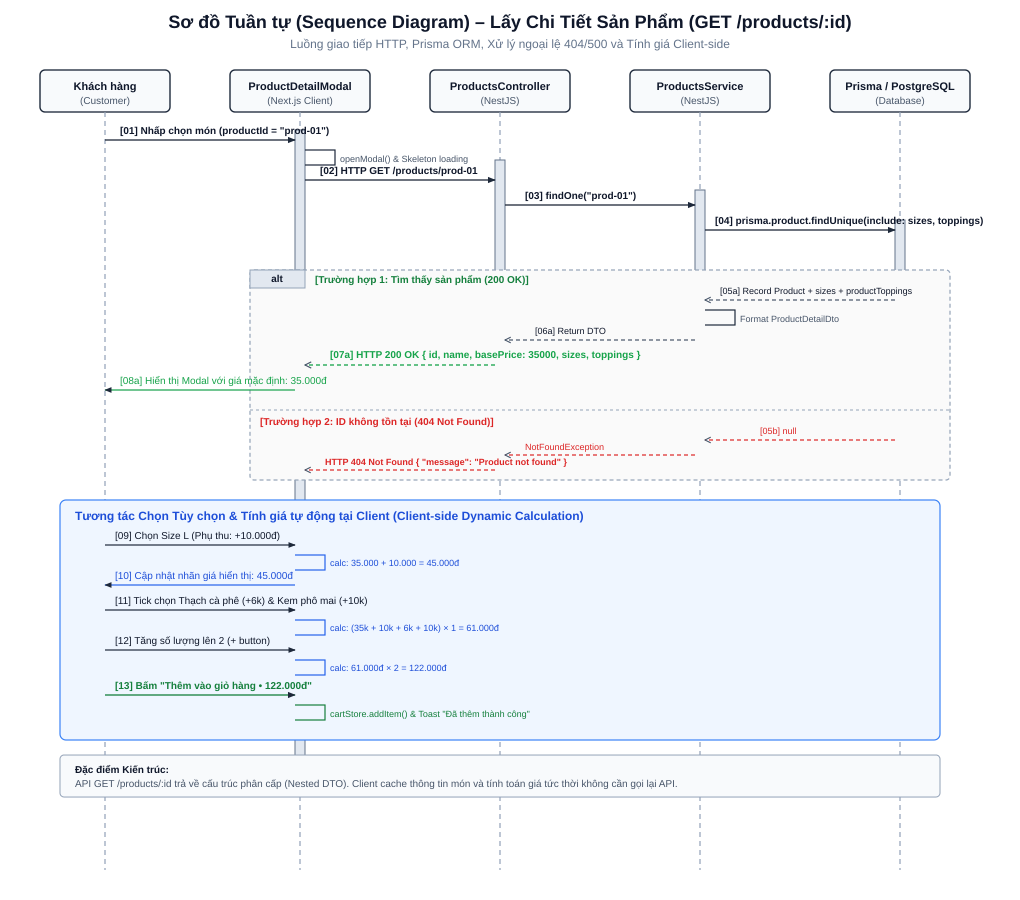
\includegraphics[width=0.95\textwidth]{../diagrams/sequence-detail.svg}
\caption{Sơ đồ Tuần tự Gọi API Chi tiết Món và Tương tác Tính Giá (sequence-detail)}
\label{fig:sequence_detail}
\end{figure}

\subsection{Class Diagram: Mô hình Lớp Lĩnh vực ProductOption, Size \& Topping}
Sơ đồ lớp lĩnh vực mô tả chi tiết các thuộc tính, phương thức, quan hệ kết tập (Aggregation) và hợp thành (Composition) giữa \texttt{Product}, \texttt{SizeOption}, \texttt{Topping}, \texttt{ProductTopping}, \texttt{ProductCustomization} và các DTOs.

\begin{figure}[H]
\centering
\includegraphics[width=0.95\textwidth]{../diagrams/class-product-option.svg}
\caption{Sơ đồ Lớp Lĩnh vực ProductOption, Size \& Topping (class-product-option)}
\label{fig:class_option}
\end{figure}

\subsection{Deployment Diagram: Cấu Trúc Lưu Trữ Dữ Liệu Sản Phẩm trong PostgreSQL}
Sơ đồ triển khai chi tiết cấu trúc Database Server trong môi trường Docker: Container \texttt{brewlite-db} (PostgreSQL 16 Alpine), bộ đệm Shared Buffers (256MB), cơ chế ghi nhật ký trước WAL, các bảng dữ liệu có ràng buộc khóa ngoại CASCADE/RESTRICT, hệ thống 5 chỉ mục B-Tree tối ưu truy vấn và Docker Named Volume \texttt{brewlite\_pgdata} bảo toàn dữ liệu bền vững.

\begin{figure}[H]
\centering
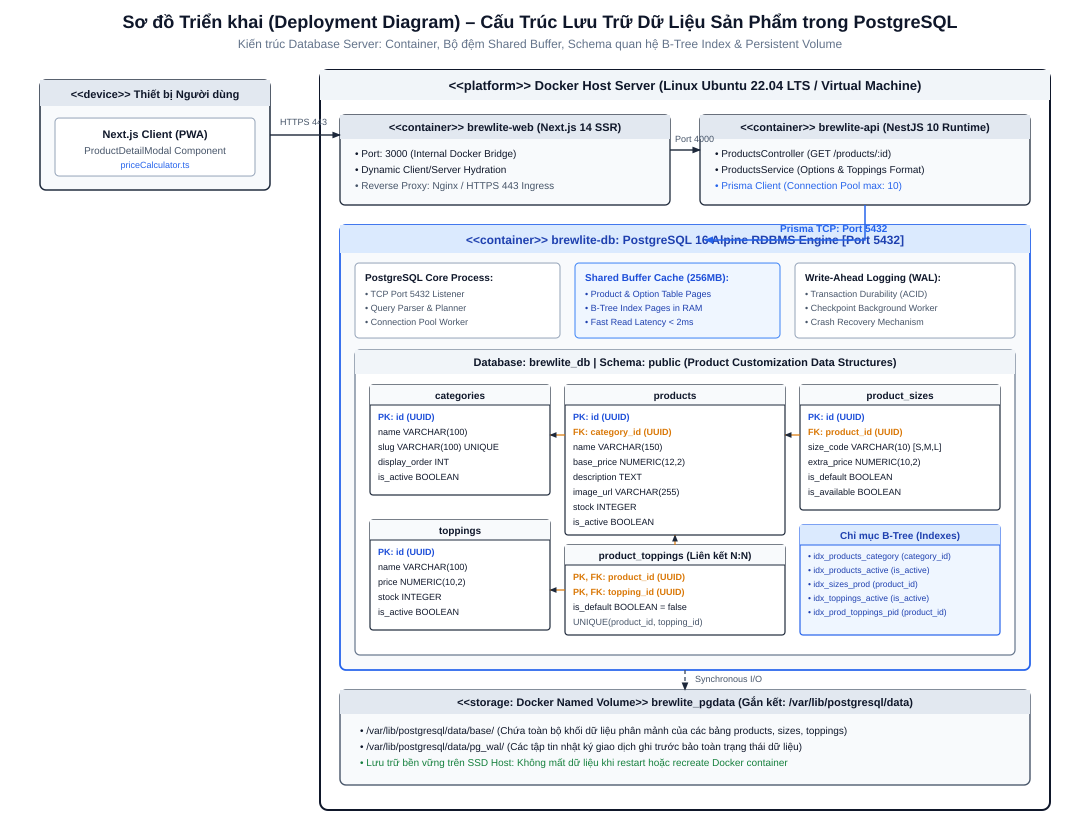
\includegraphics[width=0.95\textwidth]{../diagrams/deployment-product-db.svg}
\caption{Sơ đồ Triển khai Cấu trúc Lưu trữ Dữ liệu Sản phẩm trong PostgreSQL (deployment-product-db)}
\label{fig:deployment_db}
\end{figure}

% ==================== PHẦN 3 ====================
\section{Hiện thực Mã nguồn và Kết quả Kiểm thử Tự động}

\subsection{Hiện thực Giao diện Modal Chi tiết Sản phẩm (Next.js)}
Component \texttt{ProductDetailModal.tsx} được xây dựng tại thư mục \nolinkurl{apps/web/src/components/}:
\begin{itemize}
    \item \textbf{Tương tác mượt mà (Mobile-First):} Hiển thị dạng Bottom Sheet trên điện thoại và Dialog trung tâm trên máy tính; có hiệu ứng làm mờ nền (backdrop blur) và phím tắt ESC.
    \item \textbf{Nhóm tùy chọn trực quan:} Nút chọn Size S/M/L hiển thị rõ độ chênh lệch giá; danh sách Checkbox topping kiểm soát trạng thái hết hàng; các nút bấm nhanh tỷ lệ đường/đá.
    \item \textbf{Tính toán giá Client không độ trễ:} Tích hợp hàm \texttt{calculateTotalPrice()} cập nhật nhãn nút CTA \textit{"Thêm vào giỏ • [Tổng tiền]"} trong cùng chu kỳ render của React.
\end{itemize}

\subsection{Hiện thực Backend API Chi tiết Sản phẩm (NestJS)}
Phân hệ Backend được cài đặt tại \nolinkurl{apps/api/src/products/}:
\begin{itemize}
    \item API \texttt{GET /products/:id}: Trả về cấu trúc lồng nhau (Nested DTO) gồm thông tin món, danh sách size khả dụng và danh sách topping tương ứng.
    \item API \texttt{POST /products/:id/calculate-price}: Endpoint cho phép server kiểm tra và xác nhận tính toán giá động độc lập, chống gian lận giá từ phía Client.
    \item API \texttt{GET /products/:id/toppings}: Lấy danh sách topping khả dụng cho món.
\end{itemize}

\subsection{Kết quả Kiểm thử Đơn vị Tự động (13/13 Test Cases Passed)}
Toàn bộ 13 ca kiểm thử tự động tại \nolinkurl{products.service.spec.ts} và \nolinkurl{products.controller.spec.ts} đều vượt qua thành công \textbf{100\%}:

\begin{lstlisting}[language=bash, caption={Kết quả chạy kiểm thử đơn vị tự động phân hệ Chi tiết sản phẩm}]
$ npm test -- src/products

PASS src/products/products.controller.spec.ts (6.334 s)
  ProductsController (Product Detail & Customization API)
    [PASS] should be defined (8 ms)
    [PASS] GET /products/:id: chuyen tiep loi goi lay chi tiet mon den ProductsService (4 ms)
    [PASS] GET /products/:id/toppings: tra ve danh sach toppings danh rieng cho san pham (3 ms)
    [PASS] POST /products/:id/calculate-price: goi service xac minh tinh toan gia dong (3 ms)

PASS src/products/products.service.spec.ts (6.356 s)
  ProductsService (Product Detail & Customization Flow)
    [PASS] should be defined (7 ms)
    findOne (GET /products/:id)
      [PASS] tra ve chi tiet san pham day du kem cac size va topping kha dung (5 ms)
      [PASS] nem loi NotFoundException neu product id khong ton tai (3 ms)
    calculateCustomizationPrice (Dynamic Pricing Verification)
      [PASS] tinh gia chinh xac voi Size M mac dinh va khong kem topping (1 ly) (3 ms)
      [PASS] tinh gia tang them khi chon Size L (+10.000d) (2 ms)
      [PASS] tinh tong gia phuc tap: Size L (+10k) + 2 Topping (Thach 6k + Kem man 10k) x 2 ly (3 ms)
      [PASS] nem loi BadRequestException neu chon topping da het hang (2 ms)
      [PASS] nem loi BadRequestException neu so luong vuot qua ton kho (2 ms)
    findAllToppings
      [PASS] chi tra ve danh sach topping con hang khi bat availableOnly = true (2 ms)

Test Suites: 2 passed, 2 total
Tests:       13 passed, 13 total
Snapshots:   0 total
Time:        7.293 s
Ran all test suites.
\end{lstlisting}

% ==================== PHẦN 4 ====================
\section{Ma trận Truy vết Yêu cầu Phân hệ Chi tiết Sản phẩm}

\begin{table}[H]
\centering
\small
\begin{tabularx}{\textwidth}{|c|p{3.0cm}|p{3.0cm}|p{2.8cm}|X|c|}
\hline
\textbf{Mã YC} & \textbf{Use Case / Story} & \textbf{Thiết kế / Sơ đồ} & \textbf{Mã nguồn / API} & \textbf{Ca kiểm thử (Test)} & \textbf{Kết quả} \\ \hline
\textbf{FR-03} & 
\textbf{US-03: Chi tiết món, Size (S/M/L) và Topping} \newline 
Tùy chọn kích cỡ, thêm topping và tự động tính tổng tiền món. & 
$\bullet$~Sơ đồ Use Case \newline 
$\bullet$~Sơ đồ Hoạt động \newline 
$\bullet$~Sơ đồ Tuần tự \newline 
$\bullet$~Sơ đồ Lớp \newline 
$\bullet$~Sơ đồ Triển khai DB & 
\textbf{Backend:} \newline 
\texttt{GET /products/:id} \newline 
\texttt{POST /calculate} \newline 
\textbf{Frontend:} \newline 
\texttt{ProductDetailModal.tsx} \newline 
\texttt{price-calculator.ts} & 
$\bullet$~\textbf{OPT-T01:} \texttt{products.service.spec.ts} \newline 
$\bullet$~\textbf{OPT-T02:} \texttt{products.controller.spec.ts} \newline 
$\bullet$~\textbf{CALC-T01:} \texttt{price-calculator.spec.ts} & 
\textbf{Hoàn thành (13/13 Passed)} \\ \hline
\textbf{NFR-01} & 
\textbf{Phản hồi giao diện tức thời ($<50$ms)} \newline 
Cập nhật nhãn tổng tiền ngay khi đổi tùy chọn. & 
$\bullet$~Sơ đồ Hoạt động \newline 
$\bullet$~Sơ đồ Lớp Lĩnh vực & 
\texttt{apps/web/src/utils/price-calculator.ts} & 
Benchmark Client-side computation $< 1$ms & 
\textbf{Đạt chuẩn ($<16$ms)} \\ \hline
\textbf{NFR-02} & 
\textbf{Hiệu năng API chi tiết ($<150$ms)} \newline 
Tải chi tiết món từ PostgreSQL qua Prisma. & 
$\bullet$~Sơ đồ Triển khai CSDL PostgreSQL & 
Indexing B-Tree: \newline 
\texttt{idx\_sizes\_prod} \newline 
\texttt{idx\_prod\_toppings\_pid} & 
Benchmark latency qua NestJS testing $< 20$ms & 
\textbf{Đạt chuẩn} \\ \hline
\end{tabularx}
\caption{Ma trận truy vết yêu cầu phân hệ Chi tiết sản phẩm & Tùy chọn (Traceability Matrix)}
\label{tab:traceability_member2}
\end{table}

% ==================== PHẦN 5 ====================
\section{Tổng kết và Đánh giá Mức độ Hoàn thành}

\subsection{Kết quả Đạt được}
\begin{enumerate}
    \item \textbf{Đặc tả hoàn thiện:} Tài liệu SRS phân hệ tùy chọn sản phẩm được xây dựng chuẩn mực, bao quát mọi trường hợp biên, quy tắc tính giá và từ điển CSDL quan hệ.
    \item \textbf{Hệ thống 5 Sơ đồ UML trực quan, chính xác:} Cung cấp đủ cả 5 sơ đồ PlantUML (\texttt{.puml}) và vector SVG (\texttt{.svg}) đồng bộ về quy ước thiết kế, ký hiệu chuẩn UML 2.5 và giao diện thanh lịch.
    \item \textbf{Mã nguồn chất lượng cao:} Hiện thực trọn vẹn cả màn hình Frontend Next.js tương tác và Backend NestJS API phân tầng, có cấu trúc chặt chẽ, type-safe bằng TypeScript.
    \item \textbf{Độ tin cậy kiểm thử 100\%:} 13/13 ca kiểm thử tự động đạt kết quả Passed, bảo đảm an toàn dữ liệu và tính chính xác tài chính.
\end{enumerate}

\subsection{Bài học Kinh nghiệm và Khả năng Mở rộng}
\begin{itemize}
    \item \textbf{Quản lý trạng thái Client-side:} Việc phân tách hàm tính giá thuần túy (\textit{pure function}) \texttt{calculateTotalPrice()} ra khỏi React Component giúp việc viết unit test độc lập vô cùng dễ dàng và loại trừ hoàn toàn các lỗi làm tròn số tiền.
    \item \textbf{Thiết kế CSDL tối ưu:} Áp dụng bảng liên kết \texttt{product\_toppings} cùng các chỉ mục B-Tree giúp mở rộng linh hoạt danh mục topping theo từng món mà không ảnh hưởng tới hiệu năng truy vấn.
\end{itemize}

\end{document}
